\documentclass[10pt,a4paper]{article}
\usepackage[utf8]{inputenc}
\usepackage{graphicx}
\def\Pr{\mathop{\rm Pr}}
%\usepackage[landscape,margin=1cm]{geometry}
\usepackage[english]{babel}
\usepackage{tikz}
\usetikzlibrary{arrows,snakes,backgrounds,shapes.geometric}
\title{Probability and Statistical Inference}
\author{John S Butler}
%\date{July 2019}
\usepackage[default]{raleway}
\usepackage{fontawesome}
\usepackage[T1]{fontenc}

\usepackage{hyperref}
\usepackage{enumitem}
\usepackage{lipsum}

\usepackage{xcolor}
\definecolor{customcolor}{HTML}{616AC5}
\definecolor{alert}{HTML}{CD5C5C}
\definecolor{w3schools}{HTML}{4CAF50}
\definecolor{subbox}{gray}{0.60}
\definecolor{codecolor}{HTML}{FFC300}
\colorlet{xx}{customcolor}


%--------------------------Editor mode.

\usepackage
[citestyle=authoryear,
sorting=nty,	  		%Sorts bibliography by year, name, title
autocite=footnote, 		%Autocite command generates footnotes
autolang=hyphen, 		
mincrossrefs=1, 	
backend=biber]
{biblatex}

\DeclareFieldFormat{postnote}{#1}
\DeclareFieldFormat{multipostnote}{#1}
\DeclareAutoCiteCommand{footnote}[f]{\footcite}{\footcites}

\bibliography{literature}
%----------------------------------------
%--------------------------------------------------------------------------------
\usepackage{tcolorbox}

\tcbuselibrary{most,listingsutf8,minted}

\tcbset{tcbox width=auto,left=1mm,top=1mm,bottom=1mm,
right=1mm,boxsep=1mm,middle=1pt}

\newenvironment{mycolorbox}[2]{%
\begin{tcolorbox}[grow to left by=-1em,grow to right by=-1em,capture=minipage,fonttitle=\large\bfseries, enhanced jigsaw,boxsep=1mm,colback=#1!30!white,on line,tcbox width=auto, toptitle=0mm,colframe=#1,opacityback=0.7,nobeforeafter,title=#2]%
}{\end{tcolorbox}\\[0.2em]}

\newenvironment{subbox}[2]{%
\begin{tcolorbox}[capture=minipage,fonttitle=\normalsize\bfseries, enhanced jigsaw,boxsep=1mm,colback=#1!30!white,on line,tcbox width=auto,left=0.3em,top=1mm, toptitle=0mm,colframe=#1,opacityback=0.7,nobeforeafter,title=#2]\footnotesize %
}{\normalsize\end{tcolorbox}\vspace{0.1em}}

\newenvironment{multibox}[1]{%
\begin{tcbraster}[raster columns=#1,raster equal height,nobeforeafter,raster column skip=1em,raster left skip=1em,raster right skip=1em]}{\end{tcbraster}}

\newenvironment{textbox}[1]{\begin{mycolorbox}{customcolor}{#1}}{\end{mycolorbox}}

%-------------------------------
\newtcblisting{codebox}[2]{colback=codecolor!5,colframe=codecolor!80!black,listing only, 
minted options={numbers=left,style=tcblatex,fontsize=\tiny,breaklines,autogobble,linenos,numbersep=1mm},
left=5mm,enhanced,
title=#2, fonttitle=\bfseries,
listing engine=minted,minted language=#1}

%--------------------------------------------------------------------------------
\newcommand{\punkti}{~\lbrack\dots\rbrack~}

\renewenvironment{quote}
               {\list{\faQuoteLeft\phantom{ }}{\rightmargin\leftmargin}%
                \item\relax\scriptsize\ignorespaces}
               {\unskip\unskip\phantom{xx}\faQuoteRight\endlist}
               

%--------------------------------------------------------------------------------
\newcommand{\bgupper}[3]{\colorbox{#1}{\color{#2}\huge\bfseries\MakeUppercase{#3}}}
\newcommand{\bg}[3]{\colorbox{#1}{\bfseries\color{#2}#3}}

\newcommand{\mycommand}[2]{{\ttfamily\detokenize{#1}}~\dotfill{}~{\footnotesize #2}\\}
\newcommand{\sep}{{\scriptsize~\faCircle{ }~}}


\newcommand{\bggreen}[1]{\medskip\bgupper{w3schools}{black}{#1}\\[0.5em]}
\newcommand{\green}[1]{\smallskip\bg{w3schools}{white}{#1}\\}
\newcommand{\red}[1]{\smallskip\bg{alert}{white}{#1}\\}

\usepackage{multicol}
\setlength{\columnsep}{30pt}

\setlength{\parindent}{0pt}
\pagestyle{empty}

\usepackage{csquotes}

\newcommand{\loremipsum}{Lorem ipsum dolor sit amet.}


%--------------------------------------------------------------------------------
\begin{document}

%\maketitle
\thispagestyle{empty}
\scriptsize
%\tableofcontents


%\section{Data Type}
\section*{Network - Algorithms  (MATH1812)\footnote{\href{https://sites.google.com/dit.ie/math1812/home}{Course Website: https://sites.google.com/dit.ie/math1812/home}}}
%$\subsection*{Cheat Sheet}
\subsubsection*{\href{johnsbutler.netlify.com}{John S Butler} (TU Dublin) }

%%%% EXAMPLE Quick Find

%%% Pesudocode
\section*{Quick Find}
\begin{textbox}{Pseudocode}
\begin{subbox}{subbox}{Quick Find}
\begin{codebox}{r}{Python Pseudocode}

def Union(p,q,ID):
	pID=ID[p]
	qID=ID[q]

	if(pID==qID)
		return Connected

	 for i in range(0,10): 
		if ID[i]==pID:
			ID[i]=qID
	count=count-1	
    return ID
\end{codebox}
\end{subbox}
\end{textbox}
%%% FLOW CHART

\begin{textbox}{Flowchart }
\begin{subbox}{subbox}{Quick Find - Connecting}
\begin{center}
    
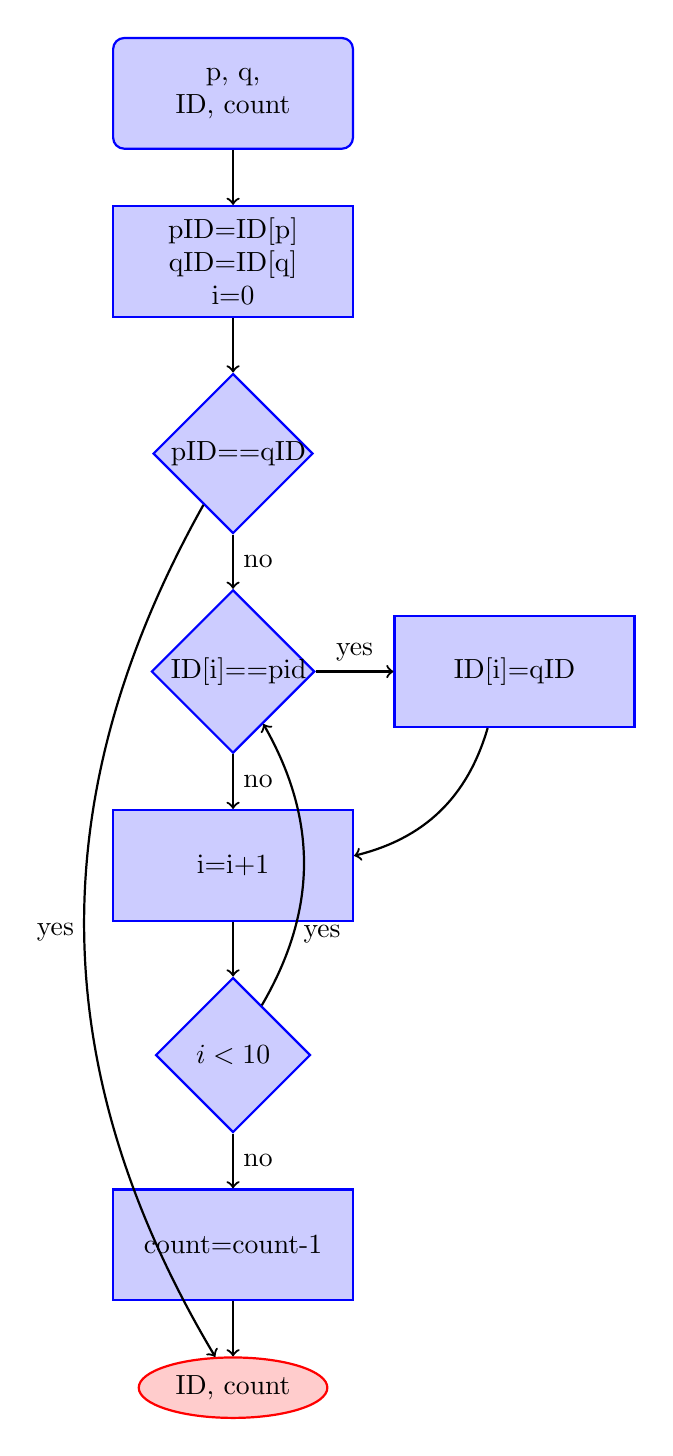
\begin{tikzpicture}[auto]
\tikzstyle{decision} = [diamond, draw=blue, thick, fill=blue!20,
text width=4.5em, text badly centered, inner sep=1pt]

\tikzstyle{block} = [rectangle, draw=blue, thick, fill=blue!20,
text width=8em, text centered, rounded corners, minimum height=4em]
\tikzstyle{block_op} = [rectangle, draw=blue, thick, fill=blue!20,
text width=8em, text centered, minimum height=4em]
\tikzstyle{line} = [draw, thick,->];
\tikzstyle{cloud} = [draw=red, thick, ellipse,fill=red!20, minimum height=2em];
\matrix [column sep=5mm,row sep=7mm]
{
% row 1
 \node [block] (init) {p, q, \\ID, count}; & \\
% row 2
\node [block_op] (identify) {	pID=ID[p]\\
	qID=ID[q]\\ i=0
}; & ;\\
\node [decision] (connect) {pID==qID}; & \\
% row 4

\node [decision] (connect2) {ID[i]==pid}; & \node [block_op] (identify3) {
ID[i]=qID};\\

\node [block_op] (identify2) {i=i+1}; & ;\\
\node [decision] (decide) {$i<10$}; & \\
\node [block_op] (identify4) {count=count-1}; & \\
% row 5
\node [cloud] (stop) {ID, count}; & \\
};
\tikzstyle{every path}=[line]
\path (init) -- (identify);
\path (identify) -- (connect);
\path (connect) -- node [midway]{no}(connect2);
\path (connect2) -- node [midway]{no}(identify2);
\path (connect2) -- node [midway]{yes}(identify3);
\path (identify3) edge [bend left]  (identify2);
\path (connect) edge [bend right] node[left] {yes} (stop);
\path (identify2) -- (decide);
\path (decide)  edge [bend right] node[near start, right] {yes}  (connect2);
\path (decide) -- node [midway] {no} (identify4);
\path (identify4) -- (stop);
\end{tikzpicture}

\end{center}
\end{subbox}

\end{textbox}

%%% Pesudocode
\section*{Quick Union}
\begin{textbox}{Pseudocode}
\begin{subbox}{subbox}{Quick Union}
\begin{codebox}{r}{Python Pseudocode Find Root}

def root(p, q, ID):
    while (p!=ID[p]):
	    p=ID[p]

    return p 


\end{codebox}


\begin{codebox}{r}{Python Pseudocode Connect}

def Union(p,q,ID,count):
	root_pID=root(p,ID)
	root_qID=root(q,ID)

	if(root_pID==root_qID):
		ID=ID
	else
    	ID[root_pID]=root_qID
    	count=count-1
	return ID


\end{codebox}
\end{subbox}
\end{textbox}
%%% FLOW CHART

\begin{textbox}{Flowchart Quick Union }
\begin{subbox}{subbox}{Flow Chart Find Root}
\begin{center}
    
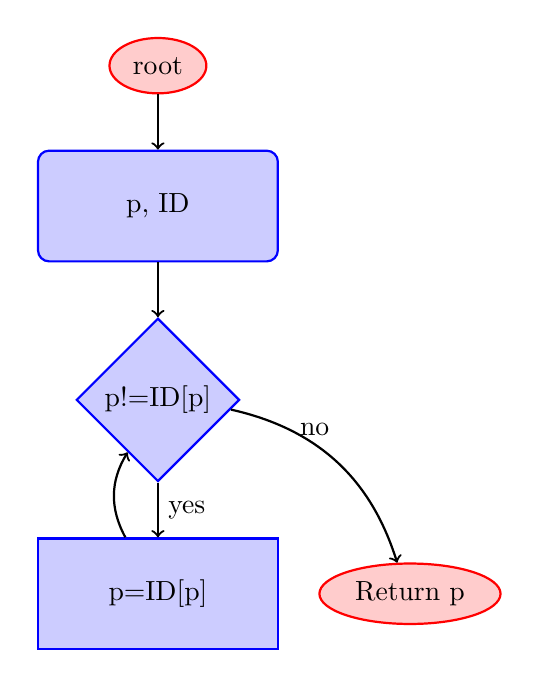
\begin{tikzpicture}[auto]
\tikzstyle{decision} = [diamond, draw=blue, thick, fill=blue!20,
text width=4.5em, text badly centered, inner sep=1pt]

\tikzstyle{block} = [rectangle, draw=blue, thick, fill=blue!20,
text width=8em, text centered, rounded corners, minimum height=4em]
\tikzstyle{block_op} = [rectangle, draw=blue, thick, fill=blue!20,
text width=8em, text centered, minimum height=4em]
\tikzstyle{line} = [draw, thick,->];
\tikzstyle{cloud} = [draw=red, thick, ellipse,fill=red!20, minimum height=2em];
\matrix [column sep=5mm,row sep=7mm]
{
% row 1
\node [cloud] (start) {root};  &;\\
\node [block] (identify) {p, ID
}; & ;\\
\node [decision] (connect) {p!=ID[p]}; & \\

\node [block_op] (identify2) {	p=ID[p]
}; & \node [cloud] (stop) {Return p};\\
};
\tikzstyle{every path}=[line]
\path (start) -- (identify);
\path (identify) -- (connect);
\path (connect) -- node [midway]{yes}(identify2);
\path (connect)edge[bend left] node[near start, right]{no}(stop);
\path (identify2)edge[bend left] (connect);
\end{tikzpicture}

\end{center}
\end{subbox}
\begin{subbox}{subbox}{Flow Chart Connect Nodes}
\begin{center}
    
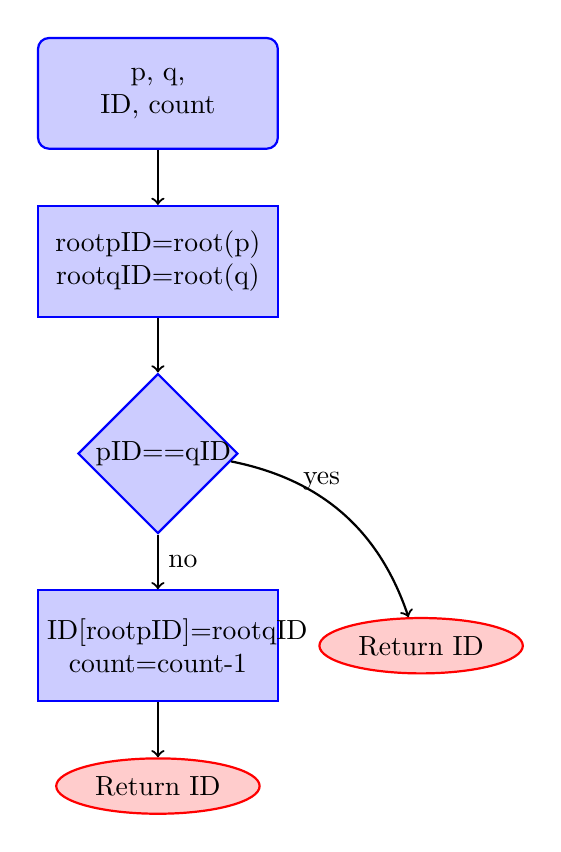
\begin{tikzpicture}[auto]
\tikzstyle{decision} = [diamond, draw=blue, thick, fill=blue!20,
text width=4.5em, text badly centered, inner sep=1pt]

\tikzstyle{block} = [rectangle, draw=blue, thick, fill=blue!20,
text width=8em, text centered, rounded corners, minimum height=4em]
\tikzstyle{block_op} = [rectangle, draw=blue, thick, fill=blue!20,
text width=8em, text centered, minimum height=4em]
\tikzstyle{line} = [draw, thick,->];
\tikzstyle{cloud} = [draw=red, thick, ellipse,fill=red!20, minimum height=2em];
\matrix [column sep=5mm,row sep=7mm]
{
\node [block] (identify) {p, q,\\ ID, count
}; & ;\\
% row 1
\node [block_op] (init) {	rootpID=root(p)\\
rootqID=root(q)
}; & ;\\
\node [decision] (connect) {pID==qID}; & \\
% row 4
\node [block_op] (stopN) {ID[rootpID]=rootqID\\ count=count-1 };&\node [cloud] (stopY) {Return ID};  \\
 \node [cloud] (stop) {Return ID };&;  \\
% row 4
};
\tikzstyle{every path}=[line]
\path (identify) -- (init);
\path (init) -- (connect);
\path (connect)-- node [midway]{no} (stopN);
\path (connect) edge[bend left] node[near start, right]{yes} (stopY);
\path (stopN) -- (stop);

\end{tikzpicture}
\end{center}
\end{subbox}

\end{textbox}



\end{document}
